\documentclass[10pt,a4paper]{article}

\usepackage[utf8]{inputenc}
\usepackage{graphicx}
\usepackage{gensymb}
\usepackage{amsmath}
\usepackage{amssymb}
\usepackage{geometry}
\usepackage{multicol}  
\usepackage{siunitx}
\usepackage{float}
\usepackage{color}
\graphicspath{{figures/}}

\geometry{a4paper}

\author{Nik Dennler \\ Johannes Lade}
\title{Digital Electronics Lab}
\date{\today{}}


\begin{document}
	
\begin{titlepage}
	\maketitle
		\begin{center}
			Email: nik.dennler@uzh.ch, johannes.lade@uzh.ch
		\end{center}
	\thispagestyle{empty}
\end{titlepage}

\tableofcontents
\newpage

\section{Catchy Introduction}
\subsection{How to build a computer?}


\section{Quick Theory}
\subsection{Digital Circuits}
Talking of circuits, we differ between analogue circuits and digital circuits. The difference lays actually in the format of the signal that represents the carried information. \newline
An analogue signal uses some attribute of the medium to convey the signal's information. In electric circuits is it the voltage, current or frequency, that is varied in order to create an electric signal. Analog electronic circuits are those in which the threshold of the current or voltage varies \underline{continuously} over time, corresponding to the information being represented. Analog circuits follow Kirchhoff's circuit laws: all the currents at a node (a place where wires meet), and the voltage around a closed loop of wires is zero. \newline
In digital electronic circuits, electric signals take on \underline{discrete values} to represent logical and numeric values, which then represent the information that is being processed. Every digital circuit is also a analog circuit, but it has (just two) discrete potential levels in use. 

\subsection{Binary Numbers}
Almost always, binary encoding is used: one voltage represents a binary '1' and another voltage, usually a value near the ground potential, represents a binary '0'. Those binary digits, each of them called one 'bit', can then be used to represent numbers and characters and therefore to carry information. The binary code was invented and first used by Gottfried Leibniz in 1679.

\begin{figure}[H]
\centering
\begin{minipage}{0.5\textwidth}
%  \centering
  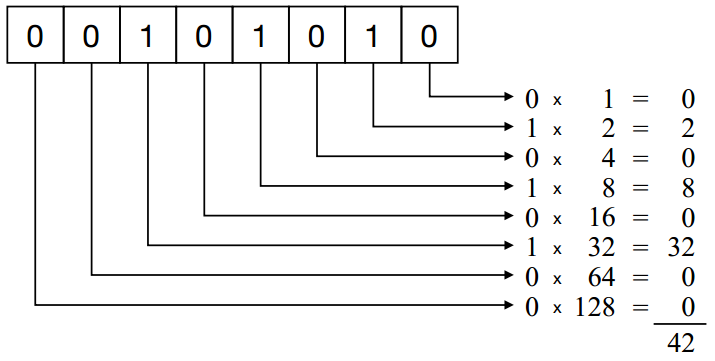
\includegraphics[width=1\textwidth]{binary.png}%
  \caption{Binary representation of one bit}%
  \label{fig:binary}
\end{minipage}%
\begin{minipage}{.4\textwidth}
  \centering
  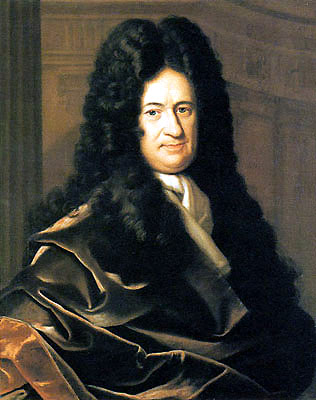
\includegraphics[width=0.8\textwidth]{leibniz}%
  \caption{Painting of Gottfried Leibniz}%
  \label{fig:leibniz}
\end{minipage}
\end{figure}

\subsection{Boolesque Algebra and its implementation}
To understand how a processor can actually perform calculations and follow algorithms with those binary numbers, some knowledge about Boolean logic has to be obtained first. We translate the digit '\texttt{1}' to \texttt{True} and the digit '\texttt{0}' to \texttt{False}. The Bool-Algebra (first half of the 19. century by George Boole) defines three main operations: 

%\noindent
\begin{itemize}
 \item \textbf{The conjunction:} $a\land b$ is $True$ if and only if $a$ is $True$ and $b$ is $True$.\\
 \item \textbf{The disjunction:} $a\lor b$  is $True$ if and only if $a$ is $True$ or $b$ is $True$ or $a\wedge b$ is $True$.\\
 \item \textbf{The negation:}  $\neg a$ is $True$ if and only if $a$ is $False$. 
\end{itemize}

\subsection{Truth tables}
These Bool operators can be represented in so called truth tables as follows. We choose here again the $1 / 0$ representation.

\begin{table}[H]
\centering
\begin{tabular}{c|c|c|c|c}
\textbf{$a$} & \textbf{$b$} & \textbf{$a\land b$} & \textbf{$a\lor b$} & \textbf{$\neg a$} \\ \hline
0          & 0          & 0            & 0            & 1           \\
1          & 0          & 0            & 1            & 0           \\
0          & 1          & 0            & 1            & 1           \\
1          & 1          & 1            & 1            & 0          
\end{tabular}
\caption{truth table}
\label{tab:truth}
\end{table}

%\noindent
The operations of the Boolean Algebra are Associative, Commutative and Distributive. They have a Neutral, an Inverse and a Zero element. One can easily imagine, that those operations can be combined and added in number to create more complex calculation operators. This is actually exactly what happens in our computers, servers and smartphones, of course on a very large scale. 

\section{Combinatoric circuits}
\subsection{General}
\subsection{Construction of a combinatoric circuit}
\subsubsection{Truth table}
\subsubsection{Equation}
\subsubsection{Draw circuit with logic elements}
\subsubsection{Unify}

\section{Sequential circuit}
\subsection{Latch}
\subsection{Construction of a sequential circuit}


\newpage
\section{Exercise Block 1}

\subsection{Exclusive OR (15min)}\label{subsec:ex-1}
\textbf{Construct an XOR gate using only the giant NAND gates.}

 XOR stands for exclusive OR. As the name suggest, it is very similar to the OR gate, except that it does not yield one when both inputs are one. In different words this means that the XOR is true whenever the two inputs are not equal. Follow the steps below to construct the XOR circuit.
\begin{enumerate}
	\item Write down the truth table.
	\item\label{it:1} Construct the disjunctive normal form from your truth table.
	\item Draw the circuit according to step \ref{it:1}.
	\item Transform the circuit in such a way that it only uses NAND Gates.
	\item Build the XOR you have drawn with the giant NAND gates.
	\item How many NAND gates do you need? See if you can loose one or two gates.
\end{enumerate}

\subsection{XOR to the Next (15min)}
\textbf{Construct the same XOR gate as in exercise \ref{subsec:ex-1} but this time with the breadboard using the tiny gates.}


\section{Excercise Block 2}

\subsection{Half-Adder (30min)}
\textbf{Build a half-adder on the bread board.}

A half-adder takes two bits $a$ and $b$ and adds them. It is called half-adder because two of them are needed in order to construct an adder which is able two add several bits. We will see later why this is the case.
\begin{table}[H]
	\centering
	\begin{tabular}{|c|c||c|c|}
		\hline
		$a$ & $b$ & $c_{out}$ & $out$ \\ \hline
		&     &           &       \\ \hline
		&     &           &       \\ \hline
		&     &           &       \\ \hline
		&     &           &       \\ \hline
	\end{tabular}
	\caption{Truth table for the Half Adder.}
	\label{tab:half-adder-truth-table}
\end{table}

\subsection{Full-Adder (30min)}

\section{Known Errors}
\subsection{Giant Logic Gates}
\begin{itemize}
	\item Check wether the power supply has a loose connection.
\end{itemize}
\subsection{Bread Board}
\begin{itemize}
	\item \textbf{Chip gets hot.} 
	\begin{itemize}
		\item You connected the power supply in the wrong direction. The chip consists of transistors i.e. diods. This means it only allows for the current to pass through the chip in one direction. Otherwise it gets grilled. Ask an assistant you'll probably have to throw it away.
	\end{itemize}
	\item \textbf{The led is not glowing.}
	\begin{itemize}
		\item Did you use the led we provided on the breadboard? It is set-up such that you don't have to think about how you have to connect it.
		\item Should it really light up? Check with the voltmeter if your gate output really is at logic one.
		\item If you really want to connect your own led think about two things. First you need to connect a $3\si{\kilo\ohm}$ resistor in series. Otherwise the led will blow. Second, remember that led stands for Light Emitting Diod. This means that you have to connect it with the longer leg towards the high voltage. 
	\end{itemize}
	\item \textbf{You forgott to connect the power supply.}
	\begin{itemize}
		\item Well I guess you know what you have to do now ;)
	\end{itemize}
	\item \textbf{Your measurements on the gate ouput don't fit your expectations.}
	\begin{itemize}
		\item What did you measure? Remember that the logic follows the voltage. In the range of $0-0.8\si{\volt}$ the output is on logic $0$. In the range of $2-5\si{\volt}$ the output is on logic $1$. The current is not affected by this and doesn't have to follow the same principle.
	\end{itemize}
\end{itemize}
\end{document}



